% basic documentclass
\documentclass[12pt]{book}

% include third party
\usepackage{ctex}
\usepackage{fancyhdr}
\usepackage{graphicx} %插入图片的宏包
\usepackage{float} %设置图片浮动位置的宏包
\usepackage{subfigure} %插入多图时用子图显示的宏包
\usepackage{hyperref}
\usepackage{geometry}

\geometry{right=2.0cm, left=2.0cm}

%% for language
\usepackage{listings}
\usepackage{xcolor}
\lstset { %
	language=C++,
	backgroundcolor=\color{black!5}, % set backgroundcolor
	basicstyle=\footnotesize,% basic font setting
}


% redefine fun
\newcommand{\icenter}[1]{\begin{center}{#1}\end{center}}
\newcommand{\isection}[1]{\begin{center}\section*{#1}\end{center}}

% basic setting
\pagestyle{fancy}

\fancyhead{}
\fancyhead[CE]{My Road To Deep Learning}
\fancyhead[CO]{\leftmark}

% title name
\title{My Road To Deep Learning}
\date{}

% document begin
\begin{document}
	
\maketitle
\thispagestyle{empty}

\newpage
\setcounter{page}{1}

%\fancyhead{}
%\fancyhead[CO,CE]{目录}

\icenter{\tableofcontents}

%%%%%%%%%%%%%%%%%%%%%%%%%%%%%%%%%%%%%%%%%%%%%%%%%%%%%%%%%%%%%%%%%%%%%%%%%%%%%%%%%%%%%%%%%%%%%%%%%%%%%%%%%
%%  第一章 绪论  %%

\newpage

\fancyhead{}
\fancyhead[CO,CE]{绪\ 论}

%\isection{第一章\ 绪\ 论}
\chapter{第一章\ 绪\ 论}
\section{一级标题}
\subsection{二级标题}
\subsection{三级标题}

\section{一级标题}

\noindent TODO:\\1. 

\newpage
this is test
 
 %%%%%%%%%%%%%%%%%%%%%%%%%%%%%%%%%%%%%%%%%%%%%%%%%%%%%%%%%%%%%%%%%%%%%%%%%%%%%%%%%%%%%%%%%%%%%%%%%%%%%%%%%
 %%  第二章 数学基础  %%
 \newpage
 
 \fancyhead{}
 \fancyhead[CO,CE]{数学基础}
 
 %\setcounter{chapter}{0}
 \chapter{第二章\ 数学基础}
 
 %\stepcounter{chapter}
 \section{高斯分布}
 一维的高斯分布(Gaussian distribution)函数表示为:
 \begin{equation}\label{eq:1d-gaussian-distribution}
G(x)=\frac{1}{\sqrt{2\pi }\sigma }e^{-\frac{(x-\mu)^{2}}{2\sigma ^{2}}}
 \end{equation}
其中$\mu$表示均值(mean),$\sigma$表示标准差(standard deviation)。一般用标准差的平方$\sigma^2$来表示方差(variance)。均值表示所有数据的平均值大小,标准差则表示数据和均值之间的偏差程度。假设所有的$N$个数据为$x_1, x_2, ..., x_n$,则均值计算方式为:
\begin{equation}\label{eq:1d-gaussian-distribution-mean}
\mu =\frac{1}{N}\sum_{i=1}^{n}x_i
\end{equation}
标准差的计算公式为:
\begin{equation}\label{eq:1d-gaussian-distribution-var}
\sigma =\sqrt{\frac{\sum \left |  x-\mu \right |^2}{N}}
\end{equation}

\begin{figure}[H]
	\centering
	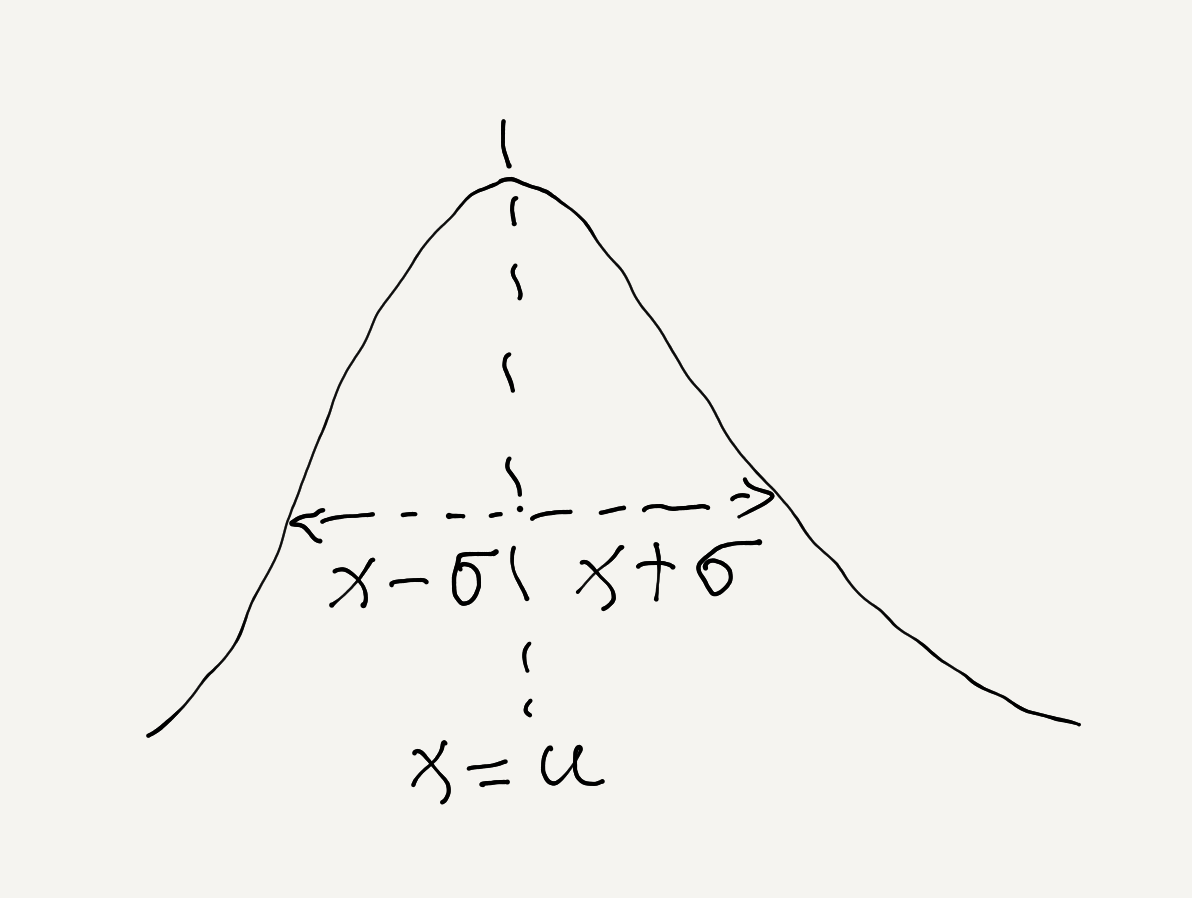
\includegraphics[width=0.7\textwidth]{images/gaussian-distribution.png}
	\caption{高斯分布函数}
	\label{gaussian-distribution} 
\end{figure}

二维高斯分布函数表示为:
 \begin{equation}\label{eq:1d-gaussian-distribution}
	G(x)=\frac{1}{2\pi \sigma ^2 }e^{-\frac{x^2 + y^2}{2\sigma ^{2}}}
\end{equation}
这里假设均值是0。

 \section{卷积}
 
 \section{距离度量}
 距离度量用来表示两个点之间的距离信息,假设有两个坐标点$(x_1, y_1), (x_2, y_2)$。则常用度量距离方式有:\\
Manhattan distance:
 \begin{equation}\label{eq:manhattan-distance}
	G = |x_1 - x_2| + |y_1 - y_2|
\end{equation}
Euclidean distance:
 \begin{equation}\label{eq:euclidean-distance}
	G = \sqrt{(x_1 - x_2)^{2} + (y_1 - y_2)^{2}}
\end{equation}

 \section{角度}
 角度(angle)和弧度(radian)换算关系为:
  \begin{equation}\label{eq:angle2radia}
 	angle = radian \times \frac{180}{\pi}
 \end{equation}
%%%%%%%%%%%%%%%%%%%%%%%%%%%%%%%%%%%%%%%%%%%%%%%%%%%%%%%%%%%%%%%%%%%%%%%%%%%%%%%%%%%%%%%%%%%%%%%%%%%%%%%%%
%%  第三章 计算机视觉  %%
\newpage
 
\fancyhead{}
\fancyhead[CO,CE]{计算机视觉}

%\setcounter{chapter}{0}
\chapter{第三章\ 计算机视觉}

%\stepcounter{chapter}
\section{相机标定}
相机标过程定主要是计算相机内参和外参的过程。一般是将现实的坐标点通过几个平面的映射关系映射到图像坐标上去\cite{computevision}。可以将转换过程分为三个部分:世界坐标系(World Coordinate System)到相机坐标系(Camera Coordinate System),相机坐标系到图像坐标系(Image Coordinate System),图像坐标系到像素坐标。整体映射过程如下:
\begin{figure}[H] %H为当前位置,!htb为忽略美学标准,htbp为浮动图形
	\centering %图片居中
	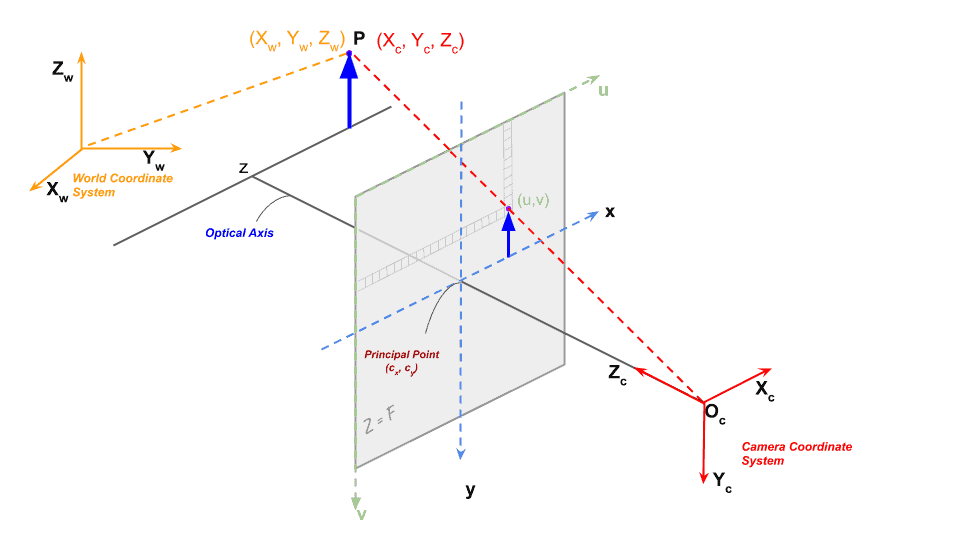
\includegraphics[width=1.0\textwidth]{images/camera-projection-3D-to-2D.png} %插入图片,[]中设置图片大小,{}中是图片文件名
	\caption{世界坐标系到像素坐标系的转换过程,图像来源\href{https://learnopencv.com/geometry-of-image-formation}{LearnOpenCV}}。 %最终文档中希望显示的图片标题
	\label{camera-projection-3D-to-2D} %用于文内引用的标签
\end{figure}

\subsection{世界坐标系到相机坐标系}
如图\ref{camera-projection-3D-to-2D},假设有一个真实三维世界坐标系 $({X_W},{Y_W},{Z_W})$ ,坐标系中的某个点坐标可表示为是 $P({X_W},{Y_W},{Z_W})$。一般情况世界坐标系的原点 $O_W$ 可选择任意位置,比如墙角处等。同理,可以以相机处的物理位置为坐标原点$O_C$得到相机坐标系 $({X_C},{Y_C},{Z_C})$,则同一个世界坐标系下的$P$点相对于相机坐标系的坐标是 $P({X_C},{Y_C},{Z_C})$, 根据相机的小孔成像原理,世界坐标系和相机坐标系下的同一点会在各个坐标方向上存在旋转和平移。


根据\cite{computevision}中公式$(2.24)$可以将两个坐标的旋转和平移表示为:
\begin{equation}\label{cv:rotatin_and_translation}
	x' = Rx + t
\end{equation}
其中$x$和$x'$是两个坐标系下的坐标,$R$是一个 $(3 \times 3)$的标准正交旋转矩阵, $t$是一个$(3 \times 1)$的平移向量。则从世界坐标系到相机坐标系的转换过程可以完整的表示为:
\begin{equation}\label{eq:rotatin_and_translation}
\left[ {\begin{array}{*{20}{c}}
		{{X_C}}\\
		{{Y_C}}\\
		{{Z_C}}
\end{array}} \right] = R \cdot \left[ {\begin{array}{*{20}{c}}
		{{X_W}}\\
		{{Y_W}}\\
		{{Z_W}}
\end{array}} \right] + t = [R|t]\left[ {\begin{array}{*{20}{c}}
		{{X_W}}\\
		{{Y_W}}\\
		{{Z_W}}\\
		1
\end{array}} \right]
\end{equation}
一般情况称旋转矩阵和平移向量的组合 $[R\ |\ t]$ 为外参矩阵(Extrinsic Matrix)。

\subsection{相机坐标系到图像坐标系}
图像坐标系图像所在平面上形成的坐标系,如图以图像中心点为坐标原点(记为$O$),以$x$为横轴,$y$为纵轴的坐标系即图像坐标系,$OO_C$则是相机的焦距$f$。$O_CP$和图像坐标系的交点坐标为$(x,y)$。 则相机坐标系到图像坐标系可以用相似变换得到。如图:
\begin{figure}[H]
	\centering
	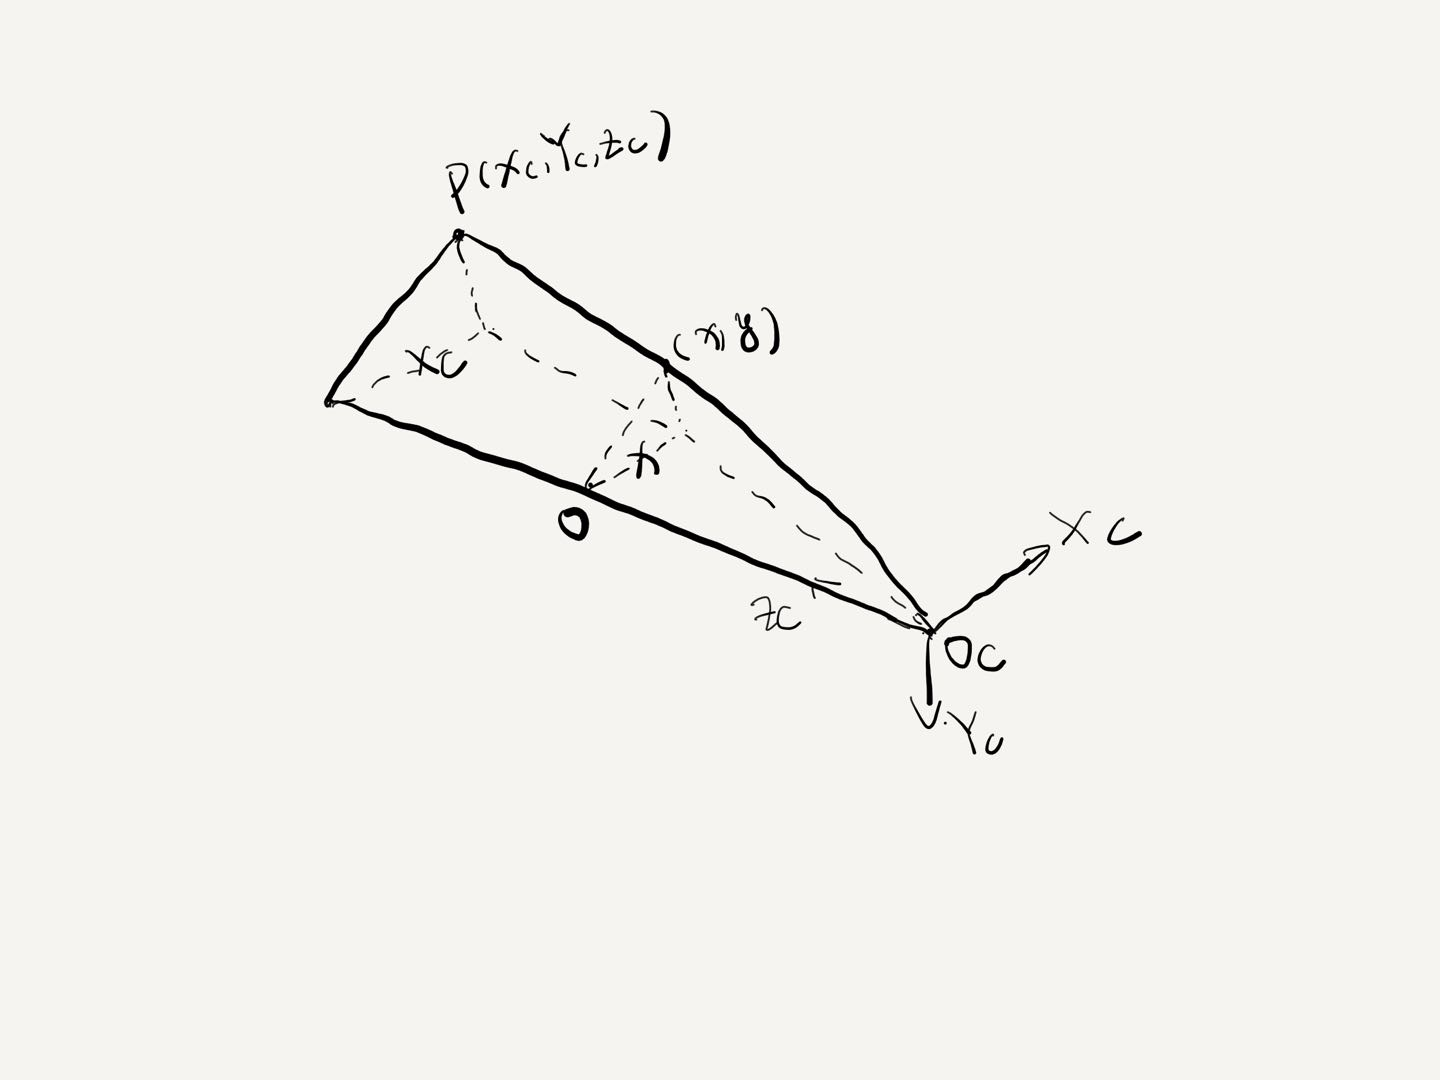
\includegraphics[width=1.0\textwidth]{images/camera_to_image_x.jpg}
	\caption{相机坐标系到图像坐标系x轴变换过程}
	\label{camera-to-image-x}
\end{figure}
由于$Z_C$轴是和图像坐标系垂直的,则根据相似三角形的变换:
\begin{equation}\label{camera_to_image_x}
\frac{x}{{{X_C}}} = \frac{{O{O_C}}}{{{Z_C}}} = \frac{{{f_x}}}{{{Z_C}}}
\end{equation}
同理,对$y$轴有$y={Y_C}{f_y}/{Z_C}$。则从坐标$P({X_C},{Y_C},{Z_C})$到$(x, y)$的变换可以用矩阵表示为:
\begin{equation}\label{camera_to_image_without_translation}
	\left[ {\begin{array}{*{20}{c}}
			{x'}\\
			{y'}\\
			{z'}
	\end{array}} \right] = \left[ {\begin{array}{*{20}{c}}
			{{f_x}}&0&0\\
			0&{{f_y}}&0\\
			0&0&1
	\end{array}} \right]\left[ {\begin{array}{*{20}{c}}
			{{X_C}}\\
			{{Y_C}}\\
			{{Z_C}}
	\end{array}} \right]
\end{equation}
其中$x=x'/z'$, $y=y'/z'$。但是一般的图像平面和相机坐标的位置没有那么标准,可能会存在一定的偏差,偏差来源有两个,一个是$Z_C$坐标轴可能不是刚好通过图像坐标系的坐标原点$O$,两者之间会有一定的偏移,记作$(c_x, c_y)$。另一个是图像平面$x$轴和$y$轴可能存在一定的旋转,不一定是垂直的。对第一种情况,在计算的时候需要考虑偏差,则公式\ref{camera_to_image_x}变成$x + {c_x} = {X_C}\frac{{{f_x}}}{{{Z_C}}}$。这里可能是加上偏差也可能是减去,$c_x$符号则有后续实际计算决定。第二种情况是模型可以简化:
\begin{figure}[H]
	\centering
	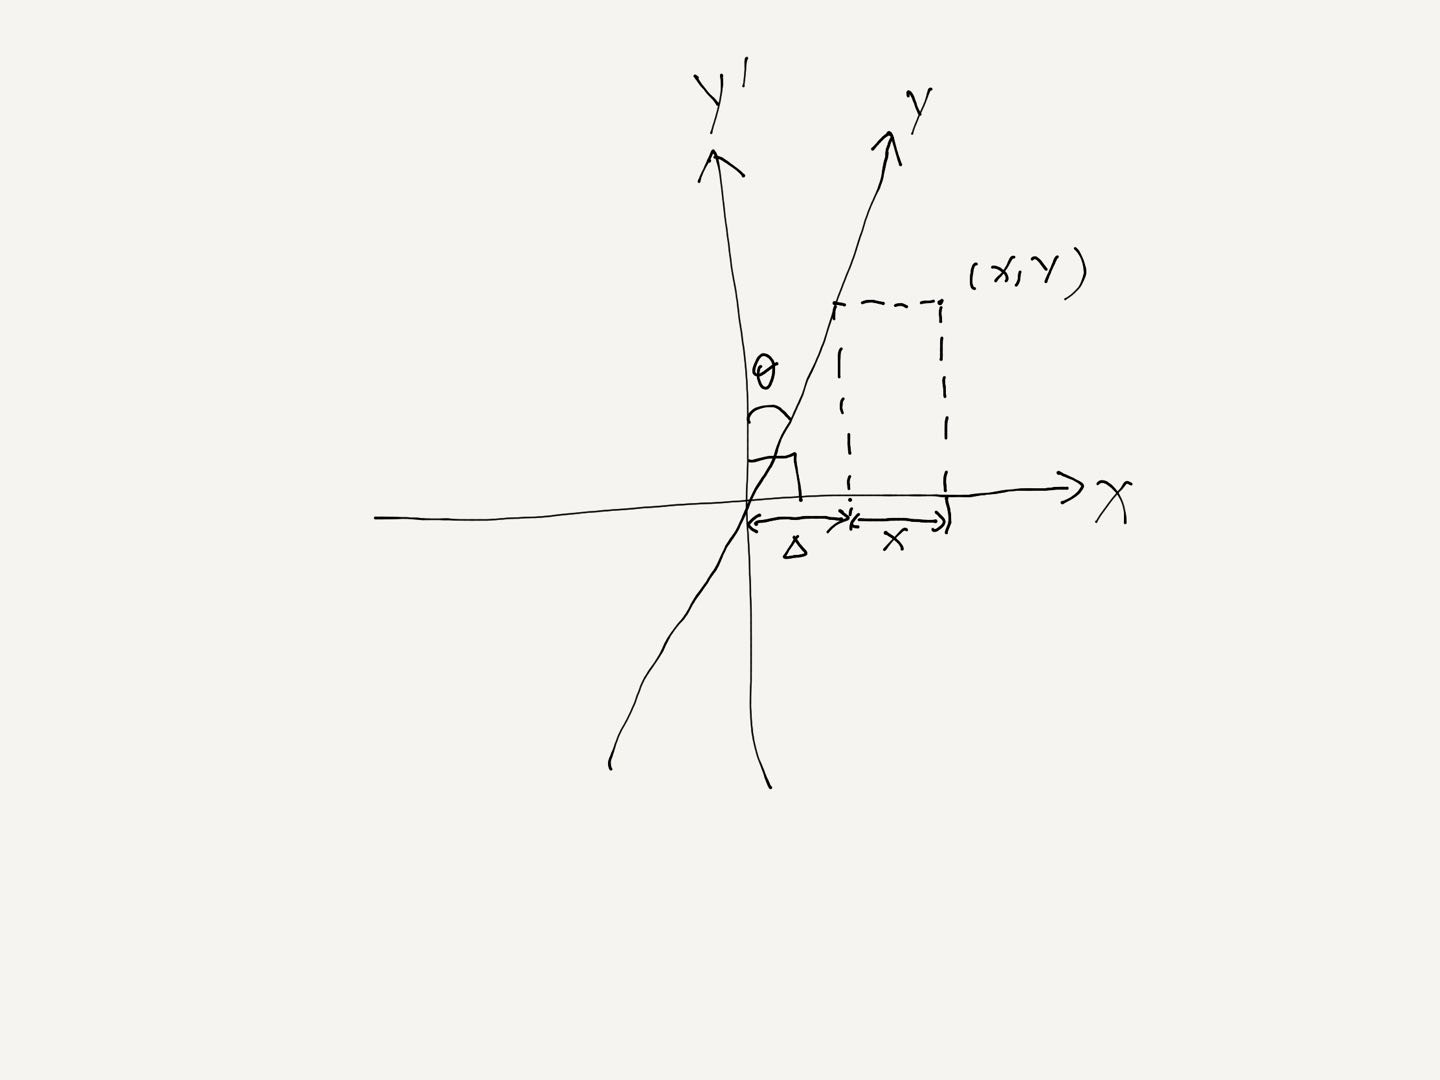
\includegraphics[width=1.0\textwidth]{images/camera_to_image_with_rotation.jpg}
	\caption{x和y轴存在一定的旋转情况}
	\label{camera-to-image-with-rotation}
\end{figure}
假设旋转角度为$\theta $,则公式\ref{camera_to_image_x}变为
\begin{equation}\label{camera_to_image_with_rotation}
\begin{array}{l}
	x = {X_C}\frac{{{f_x}}}{{{Z_C}}} + \Delta  = {X_C}\frac{{{f_x}}}{{{Z_C}}} + \tan (\theta )y\\
	\ \ = {X_C}\frac{{{f_x}}}{{{Z_C}}} + \tan (\theta ){Y_C}\frac{{{f_y}}}{{{Z_C}}}\\
	\ \ = {f_x}\frac{{{X_C}}}{{{Z_C}}} + \gamma \frac{{{Y_C}}}{{{Z_C}}}
\end{array}
\end{equation}
这里因为$\theta$和y轴的焦距$f_y$一般都是固定的,所以用$\gamma$来表示这个常数。结合以上变换最终得到相机坐标系到图像坐标系的变换矩阵为:
\begin{equation}\label{camera_to_image}
\left[ {\begin{array}{*{20}{c}}
		{x'}\\
		{y'}\\
		{z'}
\end{array}} \right] = \left[ {\begin{array}{*{20}{c}}
		{{f_x}}&\gamma &{{c_x}}\\
		0&{{f_y}}&{{c_y}}\\
		0&0&1
\end{array}} \right]\left[ {\begin{array}{*{20}{c}}
		{{X_C}}\\
		{{Y_C}}\\
		{{Z_C}}
\end{array}} \right]
\end{equation}
定义这个变换的矩阵为内参矩阵(Intrinsic Matrix)也称为相机矩阵(camera matrix)。表示为:
\begin{equation}\label{intrinsic_matrix}
K = \left[ {\begin{array}{*{20}{c}}
		{{f_x}}&\gamma &{{c_x}}\\
		0&{{f_y}}&{{c_y}}\\
		0&0&1
\end{array}} \right]
\end{equation}
其中$f_x$和$f_y$分别表示$x$轴和$y$轴上的摄像机焦距。$\gamma$是$x$轴和$y$轴之间的倾斜偏移量,$(c_x, c_y)$是像素坐标中心和相机光学中心轴$Z_C$之间的偏移值。

\subsection{图像坐标到像素坐标}
将图像坐标的坐标原点放在图像的左上角位置则变成了像素坐标,因为一般处理图像时的像素值都是以左上角为原点的。这样的话从$(x, y)$到$(u, v)$像素之间的变换就变成了线性变换:
\begin{equation}\label{pixel_translation}
\begin{array}{l}
	u = x + \frac{W}{2}\\
	v = y + \frac{H}{2}
\end{array}
\end{equation}
其中$(H, W)$表示图像的长宽,也是定值。这样可以对其变换:
\[u = x + \frac{W}{2} = {f_x}\frac{{{X_C}}}{{{Z_C}}} + \gamma \frac{{{Y_C}}}{{{Z_C}}} + {c_x} + \frac{W}{2}\]
由于$c_x$和$W/2$都是常数,可以用一下变化表示新的$c_x$
\[{c_x} \buildrel \Delta \over = {c_x} + \frac{W}{2}\]
这里如果图像坐标系的中心点和$Z_C$轴没有偏差,那么$c_x=0$,则最终得到的内参矩阵中的值$c_x=\frac{W}{2}$。所以一般可以用$W/2$来表示内参值$c_x$。

\subsection{Homography矩阵}
基于以上变化,可以到得到从点$P({X_W},{Y_W},{Z_W})$到像素$(u, v)$的变换过程:
\begin{equation}\label{world_to_pixel}
\begin{array}{l}
	\left[ {\begin{array}{*{20}{c}}
			{u'}\\
			{v'}\\
			{w'}
	\end{array}} \right] = \left[ {\begin{array}{*{20}{c}}
			{{f_x}}&\gamma &{{c_x}}\\
			0&{{f_y}}&{{c_y}}\\
			0&0&1
	\end{array}} \right]\left[ {\begin{array}{*{20}{c}}
			{{X_C}}\\
			{{Y_C}}\\
			{{Z_C}}
	\end{array}} \right]\\
\ \ \ \ \ \ \ \ \ \ = \left[ {\begin{array}{*{20}{c}}
			{{f_x}}&\gamma &{{c_x}}\\
			0&{{f_y}}&{{c_y}}\\
			0&0&1
	\end{array}} \right][R|t]\left[ {\begin{array}{*{20}{c}}
			{{X_W}}\\
			{{Y_W}}\\
			{{Z_W}}
	\end{array}} \right]
\end{array}
\end{equation}

一般为了计算会将世界坐标系的$Z_W$设为0\cite{zhang2000flexible}。则变换矩阵为:
\begin{equation}\label{homography_translation}
\begin{array}{l}
	s\left[ {\begin{array}{*{20}{c}}
			{u'}\\
			{v'}\\
			{w'}
	\end{array}} \right] = \left[ {\begin{array}{*{20}{c}}
			{{f_x}}&\gamma &{{c_x}}\\
			0&{{f_y}}&{{c_y}}\\
			0&0&1
	\end{array}} \right][\begin{array}{*{20}{c}}
		{{r_1}}&{{r_2}}&{{r_3}}&t
	\end{array}]\left[ {\begin{array}{*{20}{c}}
			{{X_W}}\\
			{{Y_W}}\\
			0\\
			1
	\end{array}} \right]\\
	s\left[ {\begin{array}{*{20}{c}}
			u\\
			v\\
			1
	\end{array}} \right] = K[\begin{array}{*{20}{c}}
		{{r_1}}&{{r_2}}&t
	\end{array}]\left[ {\begin{array}{*{20}{c}}
			{{X_W}}\\
			{{Y_W}}\\
			1
	\end{array}} \right]
\end{array}
\end{equation}

其中$r_i$是旋转矩阵的第$i$列,定义homography矩阵为:
\begin{equation}\label{homography}
H = K[R|t]
\end{equation}


对于一般的相机标定,求解内参和外参就可以变换为求解homography矩阵的形式。这里如果可以得到真实世界和像素坐标的对应点作为数据,则可以根据矩阵求解得到homography矩阵的值。但是一般真实世界的坐标不容易测量,常用的方法是使用相同的一个相机对同一个物体拍摄来获取参数,即自我标定的方法\cite{Hartley1994SelfCalibrationFM}。根据\cite{computevision}可知三维坐标系点之间的变换有旋转,平移,仿射变换,投影变换等。其中投影变换(Projective)表示为:
\[x' = Hx\]
其中$x$和$x'$表示变换前后对应的坐标点。$H$被称为透视变换矩阵或者单应性矩阵(perspective transform or homography)。

\subsection{Homography估计}
如果知道坐标点$(x, y, z)$和其经过变换后对应的坐标点$(x', y', z')$。则可以得到homography变换公式:
\begin{equation}\label{homography_two_plane}
\left[ {\begin{array}{*{20}{c}}
		{x'}\\
		{y'}\\
		{z'}two_plane
\end{array}} \right] = \left[ {\begin{array}{*{20}{c}}
		{{H_{11}}}&{{H_{12}}}&{{H_{13}}}\\
		{{H_{21}}}&{{H_{22}}}&{{H_{23}}}\\
		{{H_{31}}}&{{H_{32}}}&{{H_{33}}}
\end{array}} \right]\left[ {\begin{array}{*{20}{c}}
		x\\
		y\\
		z
\end{array}} \right]
\end{equation}

展开矩阵:
\[\frac{{x'}}{{z'}} = \frac{{{H_{11}}x + {H_{12}}y + {H_{13}}z}}{{{H_{31}}x + {H_{32}}y + {H_{33}}z}}\]
一般为了方便计算可以令$z=1$,即图像变换的时候$z$轴可以保持一致。则:
\[x'({H_{31}}x + {H_{32}}y + {H_{33}}) = {H_{11}}x + {H_{12}}y + {H_{13}}\]
\[ - x{H_{11}} - y{H_{12}} - {H_{13}} + 0 + 0 + 0 + x'x{H_{31}} + x'y{H_{32}} + x'{H_{33}} = 0\]
同理得到$y'/z'$的变换展开:
\[0 + 0 + 0 - x{H_{21}} - y{H_{22}} - {H_{23}} + y'x{H_{31}} + y'y{H_{32}} + y'{H_{33}} = 0\]
用矩阵来表示上述变换为:
\begin{equation}\label{homography_estimation}
[\begin{array}{*{20}{c}}
	{ - x}&{ - y}&{ - 1}&0&0&0&{x'x}&{x'y}&{x'}\\
	0&0&0&{ - x}&{ - y}&{ - 1}&{y'x}&{y'y}&{y'}
\end{array}]\left[ {\begin{array}{*{20}{c}}
		{{H_{11}}}\\
		{{H_{12}}}\\
		{{H_{13}}}\\
		{{H_{21}}}\\
		{{H_{22}}}\\
		{{H_{23}}}\\
		{{H_{31}}}\\
		{{H_{32}}}\\
		{{H_{33}}}
\end{array}} \right] = 0
\end{equation}
即:
\[Ah = 0\]
根据线性代数\cite{strang1993introduction}可知这是一个求解线性方程的特征向量问题。求解线性方程即可。常用的方法是将其变成对称矩阵:
\[{A^T}Ah = {A^T}0 = 0\]
然后对其进行$SVD$分解:
\[{A^T}A = U\Sigma {U^T}\]
$U$是正交矩阵,$\Sigma$是奇异值组成的对角矩阵。


\subsection{根据Homography求解旋转矩阵和平移向量}
在相机标定中常用的一种方式是将标定板先选择一个标准位置拍照,然后进行一定的旋转平移拍照。通过几次的图像来计算Homography矩阵。在上一节中可得到计算Homograohy的方法,那如果图像只有旋转和平移,homography的分解方法可参考\cite{malis2007deeper}。

\section{图像处理}
\subsection{滤波}
由于一般拍摄的图像中都含有比较多的噪声,噪声一般是图像上亮度或者颜色值随机变化的信息。比如一个小区域图像像素值都是0,但是其中一个像素值是255,那么这个点就是噪声。平滑(smooth)处理一般就是为了尽可能消除这样的噪声区域,让噪声点部分的像素值不那么明显。一般的方法是:对某一个像素点,求取以这个像素点为中心的局部区域的像素值的加权像素值,然后用新的像素值来代替之前的像素值。这种减小噪声的方法称为滤波(filter)。常见的滤波方式有均值滤波和高斯滤波,均值滤波是在计算新的像素值的时候将区域内的所有像素值求平均,这种操作一般则可以通过卷积的方式来实现,比如:
\begin{figure}[H]
	\centering
	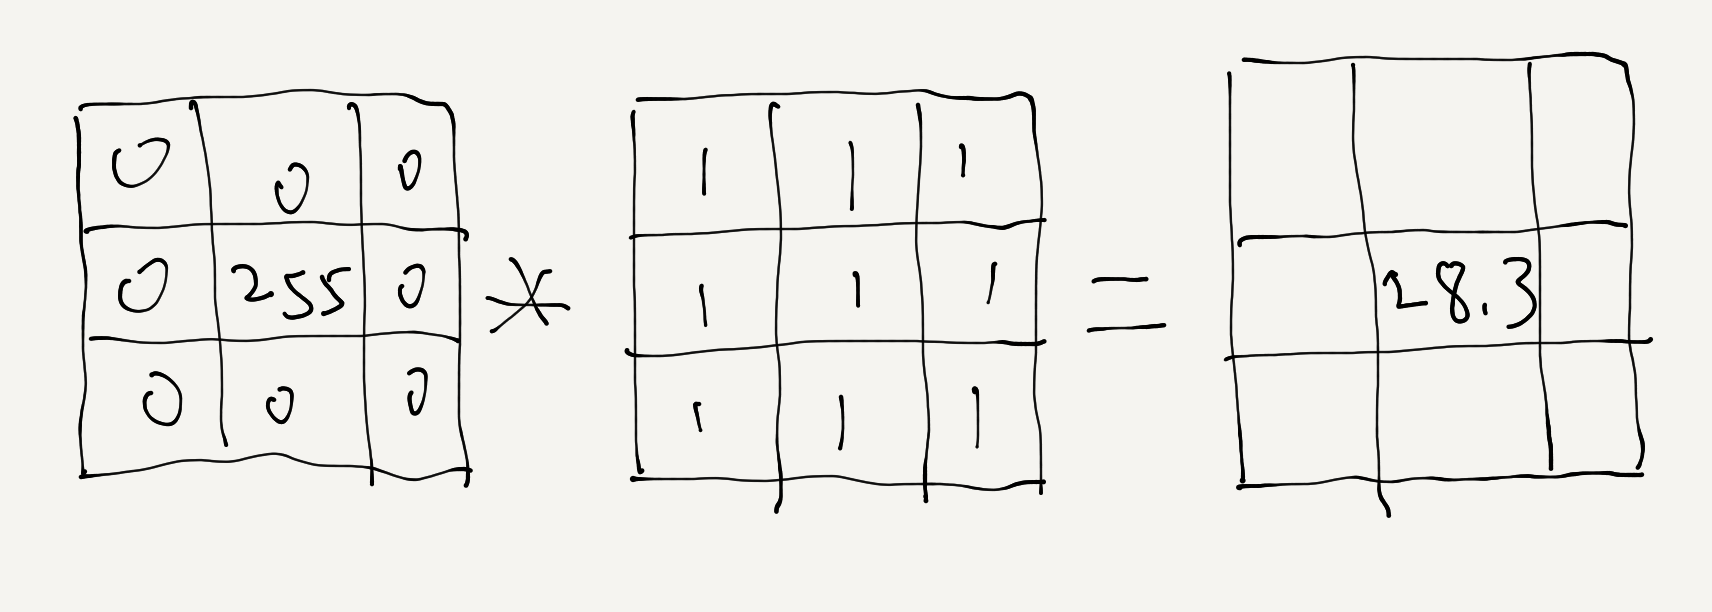
\includegraphics[width=0.7\textwidth]{images/mean-filter.png}
	\caption{均值滤波卷积}
	\label{mean-filter} 
\end{figure}
通过使用一个$3x3$的卷积核对原始图像进行计算,之前的255的像素值就变成了28.3。这样就使得像素值差别没有之前那么明显,整张图像看起开也变得更加平滑。另一种常用的滤波方式是高斯滤波,像均值滤波里使用了全是1的卷积核一样,高斯滤波的区别是使用一个具有高斯分布的卷积核。卷积核的目的主要是作为像素的权重值,那么对于某个点我们一般是希望这个点的权重要比周围像素点权重大的,这样可以尽可能的保留像素的原始信息。而高斯分布则正是中心点概率值大,周围概率值小,所以高斯滤波具有更好的效果。由于图像是二维的,所以一般需要二维高斯分布函数生产一个二维的卷积核。

%%%%%%%%%%%%%%%%%%%%%%%%%%%%%%%%%%%%%%%%%%%%%%%%%%%%%%%%%%%%%%%%%%%%%%%%%%%%%%%%%%%%%%%%%%%%%%%%%%%%%%%%%
\newpage

\fancyhead{}
\fancyhead[CO,CE]{深度学习}

%\setcounter{chapter}{0}
\chapter{第四章\ 深度学习}
本章主要叙述深度学习及机器学习基础及部分网络结构。

\section{机器学习}
\subsection{K-MEAN}
\section{分类模型}
\section{检测模型}
\section{分割模型}
\section{量化}
假设将float区间$x_{float}^{min}\sim x_{float}^{max}$,量化表示区间为:$x_{quantized}^{min}\sim x_{quantized}^{max}$,则量化公式为:
\[scale = \frac{x_{float}^{max} - x_{float}^{min}}{x_{quantized}^{max} - x_{quantized}^{min}}\]
\[position = x_{quantized}^{max} - \frac{x_{float}^{max}}{scale}\]
\[x_{quantized} = \frac{x_{float}}{scale} + position\]


%%%%%%%%%%%%%%%%%%%%%%%%%%%%%%%%%%%%%%%%%%%%%%%%%%%%%%%%%%%%%%%%%%%%%%%%%%%%%%%%%%%%%%%%%%%%%%%%%%%%%%%%%
\newpage

\fancyhead{}
\fancyhead[CO,CE]{算法}

%\setcounter{chapter}{0}
\chapter{第五章\ 算法}
\section{复杂度计算}
时间复杂度可表示为: $O(1), O(n), O(logn)$等,表示完成计算需要进行的次数。
\begin{lstlisting}
std::unordered_map<int, int> map;
int value = map[0];   // O(1)-> hash map get outputs only once

for (int i = 0; i < n; ++i) {
 // ... for loop n -> O(n)
}

// O(logn)
std::vector<int> nums{1, 2, 3, 4, 5, 6, 7, 8};
// if search for 2
// first dichotomy: 1, 2, 3, 4, size = 8 * (1/2)  = 4
// second dichotomy: 1, 2, siz = 8 * (1/2) * (1/2) = 2
// third dichotomy: 2,  size = 8 * (1/2) * (1/2) * (1/2) = 1
\end{lstlisting}
$O(logn)$是比较不容易理解的,如代码一个数组使用二分法查找某一个数字,长度为8的数字需要进行三次二分才可以找到对应的值。那么假设有$n$个数字,需要经过$k$次二分可以找到值。则有:$n * (1/2)^k = 1$,即$k$次查找之后数组长度是1。log变化之后:
\begin{equation}\label{log-algorithm-time}
k = log_2(n)
\end{equation}
这称为对数时间,即为$O(logn)$.(这里统一记作logn而不用管log的底是多少,因为根据换底公式,不同的底数只是一个常系数的差别)。比如长度为8带入公式得到k是3,即最多进行三次运算就可以找到对应的值了。

\section{排序算法}
\subsection{拓扑排序}
对一个有向无环图,可以通过拓扑排序获取图上每个节点的执行顺序。假设对一个节点定义如下:
\begin{lstlisting}
struct Node {
 public:
  Node(std::string name) : name_(name) {}
  void add(Node* node) {
	++(node->in_degree);
	next_nodes.emplace_back(node);
  }
  int in_degree = 0;
  std::vector<Node*> next_nodes;
	
  std::string name_;
};
\end{lstlisting}
节点包含一下信息: 入度(in\_degree)表示当前节点的输入节点个数。next\_nodes表示当前节点的所有输出节点。拓扑排序的思想为:当一个节点的入度是0的时候则可以执行当前节点(将节点放入queue中),同时可以从图上删除当前节点,并且将节点的所有next\_nodes的入度都减去1。同样的方法遍历完所有的节点即可得到一个可执行队列。

\subsection{快速排序}
快速排序方法:
先选一个基准数,然后从数组尾地址向前,如果值小于基准值,则将值移动到基准前面。同时从开始位置向后移动,如果值大于基准值,则将值移动到基准值后面。这样一次排序得到了基准值在数组中的位置,然后使用分治加上递归思想。分别对基准位置前面的数组和后面的数组再次进行排序。调用递归函数直到起始位置等于终止位置。
\begin{lstlisting}
void quick_sort(std::vector<int>& nums, int start, int end) {
  if (end < start) return;
	int base = nums[start];
	int index = start;
		
	int i = start;
	int j = end;
	while (i < j) {
		while (i < j && nums[j] >= base) {
			j--;
		}
		nums[i] = nums[j];   // set nums[j] before base, set it to index i
		while (i < j && nums[i] <= base) {
			i++;
		}
		nums[j] = nums[i];  // set nums[i] after base, set it to index j
		nums[i] = base;   // i == j, set nums[i] == base, set base in middle
	}
	quick_sort(nums, start, i - 1);
	quick_sort(nums, i + 1, end);
}
\end{lstlisting}

\section{Graph}
\subsection{DFS and BFS}
Depth First Search Algorithm(DFS),深度优先搜索算法:从某一个节点开始,沿着一条搜索路径一直走到底,如果不满足条件然后从这条路尽头的节点回退到上一个节点,再从另一条路开始走到底。依次按照这种规律递归所有的节点。Breadth-First Search (BFS) 广度优先搜索,从根节点开始,分别搜索左右节点,左右节点不满足条件在分别搜索左节点的子节点和右节点的子节点,依次遍历所有节点。对输入节点:
\begin{figure}[H]
	\centering
	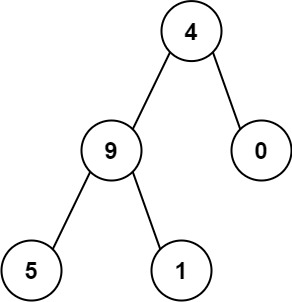
\includegraphics[width=0.7\textwidth]{images/num2tree.jpg}
	\caption{node-tree}
	\label{node-tree-dfs-bfs}
\end{figure}
dfs和bfs算法如下:
\begin{lstlisting}
#include <iostream>
#include <vector>
#include <queue>

struct TreeNode {
	int val;
	TreeNode *left;
	TreeNode *right;
	TreeNode() : val(0), left(nullptr), right(nullptr) {}
	TreeNode(int x) : val(x), left(nullptr), right(nullptr) {}
	TreeNode(int x, TreeNode *left, TreeNode *right) : val(x), left(left), right(right) {}
};

void dfs(TreeNode* root) {
	if(nullptr == root) return;
	dfs(root->left);
	std::cout << root->val << " -> ";
	dfs(root->right);
}

void bfs(TreeNode* root) {
	if (root == NULL)
	return;
	std::queue<TreeNode*> q;
	q.push(root);
	while (!q.empty()) {
		TreeNode* node = q.front();
		std::cout << node->val << " -> ";
		q.pop();
		
		if (nullptr != node->left) q.push(node->left);
		if (nullptr != node->right) q.push(node->right);
	}
}


int print(TreeNode* root) {
	dfs(root);
	std::cout << "\n";
	
	bfs(root);
	std::cout << "\n";
}

int main() {
	TreeNode n0(0);
	TreeNode n1(1);
	TreeNode n5(5);
	TreeNode n9(9, &n5, &n1);
	TreeNode n4(4, &n9, &n0);
	int sum = print(&n4);
}
\end{lstlisting}
dfs输出节点: $5 \rightarrow 9 \rightarrow 1 \rightarrow 4 \rightarrow 0$\newline
bfs输出节点: $4 \rightarrow 9 \rightarrow 0 \rightarrow 5 \rightarrow 1$\newline

%%%%%%%%%%%%%%%%%%%%%%%%%%%%%%%%%%%%%%%%%%%%%%%%%%%%%%%%%%%%%%%%%%%%%%%%%%%%%%%%%%%%%%%%%%%%%%%%%%%%%%%%%
\newpage

\fancyhead{}
\fancyhead[CO,CE]{计算机基础}

%\setcounter{chapter}{0}
\chapter{第六章\ 计算机基础}
\section{基础概念}
\subsection{计算机体系结构}
中央处理器(CPU,Central Processing Unit)是一块超大规模的集成电路,结构如下:
\begin{figure}[H]
	\centering
	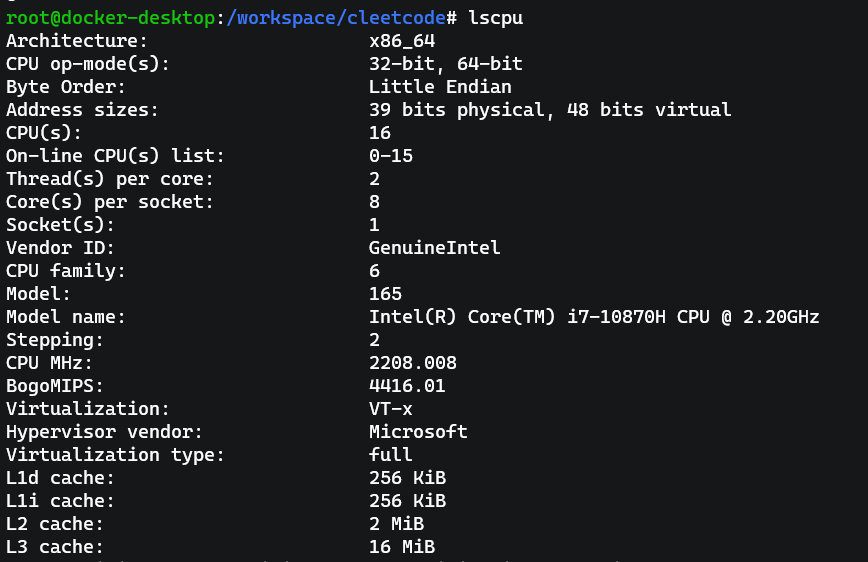
\includegraphics[width=0.7\textwidth]{images/cpu_architecture.png}
	\caption{Cpu-diagram}
	\label{Cpu-diagram}
\end{figure}

查看系统版本:
\begin{figure}[H]
	\centering
	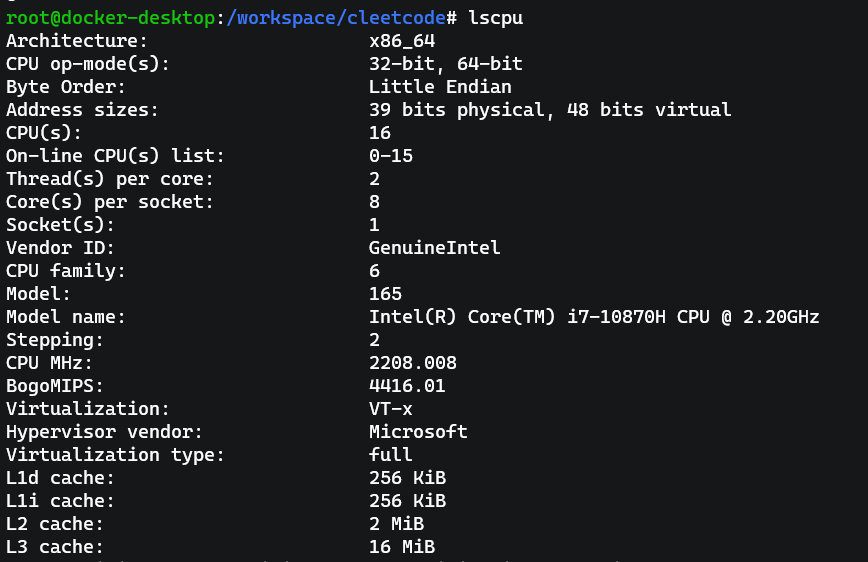
\includegraphics[width=0.7\textwidth]{images/cpu_architecture.png}
	\caption{计算机Architecture}
	\label{cpu-architecture}
\end{figure}
参数解析:\newline
\begin{itemize}
\item[$\bullet$] Architecture: x86\_64表示是64位系统,x86\_32表示32位系统。
\item[$\bullet$] CPU op-mode: 表示Linux在运行什么系统的版本,64位系统支持32以及64位的系统程序。
\item[$\bullet$] CPU: 一共有多少个CPU
\end{itemize}

\subsection{程序编译原理}
程序编译步骤包括:
 \begin{center} 源文件 $\rightarrow$ 预处理器 $\rightarrow$ 编译器 $\rightarrow$ 连接器 $\rightarrow$ 目标机器代码 \end{center}
预处理器: 完成将多个源文件汇聚在一起的任务,主要包括将头文件代码copy到源文件中,将对应的宏进去扩展开。\\
编译器: 完成预处理后文件到汇编语言的转换。(编译器包括语法分析、代码生成等步骤)\\
汇编器: 将汇编程序生成可重定位的机器代码。\\
链接器: 将多个编译文件链接在一起。\\
\subsection{bandwidth and throughput}
带宽(bandwidth)是数据传输的最大速率;
吞吐量指单位时间内运算/传输的数据量

\subsection{内存}
计算机中存储速度从快到慢依次是: 寄存器->缓存->主存->磁盘存储器。CPU和GPU的主存都采用的是DRAM(动态随机存取存储器)。

\section{常用命令工具}
\subsection{Windows}
\subsection{Ubuntu}
\textbf{创建虚拟环境}
\begin{lstlisting}[language=bash]
# virtualenv
which python3.7
virtualenv venv -p /usr/bin/python3.7
\end{lstlisting}

%%%%%%%%%%%%%%%%%%%%%%%%%%%%%%%%%%%%%%%%%%%%%%%%%%%%%%%%%%%%%%%%%%%%%%%%%%%%%%%%%%%%%%%%%%%%%%%%%%%%%%%%%
\newpage

\fancyhead{}
\fancyhead[CO,CE]{c++}

%\setcounter{chapter}{0}
\chapter{第七章\ c++}

\section{基础概念}
\subsection{const}
const用来修饰变量或者函数为不可变的,但在不同地方意思不同:
\begin{lstlisting}
int* const ptr = new int[4];  //  pointer const
const int* ptr;  //  const pointer
\end{lstlisting}
指针常量: 指针指向的地址不能被改变,即指针对象不能被修改。但是指针指向的内容是可以修改的。并且可以cast成void*,注意这里cast之后指针地址还是没有被改变的,只是类型变成void*了。指针变量中const修饰的是变量值,即这个变量值不能被修改,但是前面的指针是可以被操作的。指针常量在定义时必须被初始化,所以一般在class中如果有指针常量则必须在构造的时候使用初始化列表来初始化指针常量:
\begin{lstlisting}[language=C++]
int* const ptr = new int[4];
// valid:
ptr[0] = 1;
void* void_ptr = static_cast<void*>(ptr);

// invalid
int* new_data = new int[4]; // invalid if set new data to ptr, ptr = new_data;


// in class
class A {
 public:
  A(int* data) : data_(data) {}
  //A() {
  //  data_ = new int[1];  // invalid init in here
  // }
	
 private:
  int* const data_;  // must init in initialize list 
};
\end{lstlisting}
常量指针: 返回的指针不能被修改,比如cast成void*等。并且指针指向的值也是不可以修改的。常量指针定义时可以不用初始化。但是同一个指针变量可以指向新的指针位置,因为常量指针修饰的时指针地址(int*),即不允许对这个指针地址操作。但是指针变量(ptr)是可以被改变的。
\begin{lstlisting}
// valid
const int* ptr;
ptr = new int[4];
ptr = new int[10];  // valid to change to pointr address for ptr;

// invalid
// ptr[0] = 1;  // invalid
// void* void_ptr = static_cast<void*>(ptr);  // invalid to cast it
\end{lstlisting}

const修饰函数,在函数声明后用关键字const表示的"const function",常量函数内只能对成员变量进行读操作,不能修改成员变量,如果修改了则会出现编译期报警。但是如果是函数内的零时变量是可以修改的。const修饰类A时表示类的方法都是不可修改的,所以调用aa的时候只能调用其常量成员函数,不允许调用其非const成员函数add,在const对象上调用了一个非const成员函数,这是不允许的,因为非const成员函数没有承诺不修改对象,所以编译器会做一个安全的假设,add()可能会试图修改对象,但是aa又是const的不能被修改所以此时编译器会编译报错。
\begin{lstlisting}
class A {
 void log() const;  // const function
 void add();
};

const A aa;
aa.log();
aa.add();  // invalid
\end{lstlisting}

\subsection{字符}
c++中单引号表示字符,双引号表示字符串。

\begin{lstlisting}
std::string a = "a";
char b = 'b';
// if ('a' == a) // invalid, for a is tring, but 'a' is const char
std::cout << typeid(a).name() << " " << typeid(b).name() << " " << typeid(a[0]).name() << "\n";
// output is: OKNSt7__cxx1112basic_stringIcSt11char_traitsIcESaIcEEE c c
// first a is string type, b and a[0] is c(char).
\end{lstlisting}

对于char类型来说,常用的char对应的ASCII码是:
\begin{lstlisting}{language=bash}
Dec  Char                           Dec  Char     Dec  Char     Dec  Char
---------                           ---------     ---------     ----------
0  NUL (null)                      32  SPACE     64  @         96  `
1  SOH (start of heading)          33  !         65  A         97  a
2  STX (start of text)             34  "         66  B         98  b
3  ETX (end of text)               35  #         67  C         99  c
4  EOT (end of transmission)       36  $         68  D        100  d
5  ENQ (enquiry)                   37  %         69  E        101  e
6  ACK (acknowledge)               38  &         70  F        102  f
7  BEL (bell)                      39  '         71  G        103  g
8  BS  (backspace)                 40  (         72  H        104  h
9  TAB (horizontal tab)            41  )         73  I        105  i
10  LF  (NL line feed, new line)    42  *         74  J        106  j
11  VT  (vertical tab)              43  +         75  K        107  k
12  FF  (NP form feed, new page)    44  ,         76  L        108  l
13  CR  (carriage return)           45  -         77  M        109  m
14  SO  (shift out)                 46  .         78  N        110  n
15  SI  (shift in)                  47  /         79  O        111  o
16  DLE (data link escape)          48  0         80  P        112  p
17  DC1 (device control 1)          49  1         81  Q        113  q
18  DC2 (device control 2)          50  2         82  R        114  r
19  DC3 (device control 3)          51  3         83  S        115  s
20  DC4 (device control 4)          52  4         84  T        116  t
21  NAK (negative acknowledge)      53  5         85  U        117  u
22  SYN (synchronous idle)          54  6         86  V        118  v
23  ETB (end of trans. block)       55  7         87  W        119  w
24  CAN (cancel)                    56  8         88  X        120  x
25  EM  (end of medium)             57  9         89  Y        121  y
26  SUB (substitute)                58  :         90  Z        122  z
27  ESC (escape)                    59  ;         91  [        123  {
28  FS  (file separator)            60  <         92  \        124  |
29  GS  (group separator)           61  =         93  ]        125  }
30  RS  (record separator)          62  >         94  ^        126  ~
31  US  (unit separator)            63  ?         95  _        127  DEL
\end{lstlisting}
这里字符'0'对应的整型数是48,所以一般可以通过如下方式将char类型转成整形:
\begin{lstlisting}
std::cout << int('0');   // 48
int number = '5' - '0';  // 5, '5'-'0' it evaluates to 53-48, or the int 5
\end{lstlisting}
字符的加减运算可替换成整型数的加减运算。

\subsection{类型别名}
类型别名(type alias)可以使用关键字typedef或者using,用来表示将某个类型重命名。
\begin{lstlisting}
typedef type new_name;
using new_name = type;
\end{lstlisting}

\subsection{typename}
在模板声明的模板参数列表中,typename可以替代class来声明类型模板参数和模板模板参数。
\begin{lstlisting}
template <typename T>
\end{lstlisting}
在模板内,如果要使用一个依赖于模板参数的类型,则需要用typename来说明,参考c++标准:A name used in a template declaration or definition and that is dependent on a template-parameter is assumed not to name a type unless the applicable name lookup finds a type name or the name is qualified by the keyword typename。
\begin{lstlisting}
template <typename T>
struct A {
  typedef typename T::Type type;
};
\end{lstlisting}
这里要使用模板参数T的一个类型Type并用typedef将其命名为type。但是由于是一个依赖类型(Dependent names),即Type依赖传入的模板参数T。但是T是一个未知的类型,所以是不清楚Type的具体含义的,比如是类型还是静态成员变量什么的。所以需要加上typename来修饰让编译清楚这是一个数据类型,从而编译时才不会出错。

\subsection{函数原型}
函数原型( function prototype)是函数的声明,它告诉程序函数返回值的类型以及参数的数量和类型。函数类型需要在头文件中进行定义然后在cpp文件中实现函数定义。函数原型中的名字是可选的可以省略,即参数的名字是可以省略的。
\begin{lstlisting}
void fun(int a);
void fun(int);
void fun(int a = 1);
\end{lstlisting}

\subsection{namespace}
\begin{lstlisting}
namespace {}
\end{lstlisting}

\subsection{decltype}
\subsection{extern}
\subsection{volatile}
volatile关键字表示修饰的对象可能会被改变,不需要编译器进行优化。比如:
\begin{lstlisting}
int value = 12581;

while(value == 12581)
{
  // ...
}
\end{lstlisting}
这种情况编译器会将其优化成while(true)的形式,但是实际上value可能会被其它编译器感知不到的地方所改变其值。这种情况就不希望编译器优化value。则可以通过添加volatile关键字来告诉编译器不要优化修饰的对象。

\subsection{函数指针}
\subsection{noexcept}
函数
\subsection{restrict}
\subsection{value initialization}
\subsection{预处理命令}
\#pragma

\subsection{操作符}
$\land$ \newline
c++中,$\land$ 表示异或(XOR)操作,运算的规则是相同为0,不同为1。
\begin{lstlisting}
1 ^ 1 = 0;  1 ^ 0 = 1; 0 ^ 0 = 0; 1 ^ 2 = 3;
\end{lstlisting}

\% \newline
\%表示两个数的余数值, /表示两个数相除的整数部分。比如11除3整除部分是3余数是2。
\begin{lstlisting}
11 % 3 = 2;
11 / 3 = 3;
\end{lstlisting}

\subsection{类型转换}
\textbf{reinterpret\_cast} \newline
reinterpret\_cast只能执行指针到指针的转换和引用到引用的转换(加上指针到整型和整型到指针的转换)。使用reinterpret\_cast是一种比较危险的转换方式,比如转换两个指针,reinterpret\_cast会根据指针类型强制转换指针指向值的bit位含义,但是却不改变指针本身,并且在编译期不会做类型检查也不会报错。所以reinterpret\_cast一般只用于普通指针转成void*或者将void*转成指针原本表示的数据类型。
\begin{lstlisting}
int num = 48;
int* int_ptr = &num;
char* str_ptr = reinterpret_cast<char*>(int_ptr);

std::cout << int_ptr << " " << static_cast<void*>(str_ptr) << "\n";
// 0x7ffff93397a4 0x7ffff93397a4

std::cout << *int_ptr << " " << *str_ptr << "\n";
// 48 0

float* float_ptr = reinterpret_cast<float*>(int_ptr);
std::cout << float_ptr << " " << *float_ptr << "\n";
// 0x7ffff93397a4 6.72623e-44

// next is invalid, compiler error for cast is not ptr or reference
double b = reinterpret_cast<double>(num);  
\end{lstlisting}
从测例可以看出,使用reinterpret\_cast对指针转换后指针地址是都没有改变的,但是指针指向的值确完全不一样,当是int*时,指针指向的时int类型,表示数字是48,当转换成char*时指针指向的时char类型,编译器解析的时候按照char类型来存储读取对应的值,48则对应了char里面的'0'。当转成float*的时候,这就是一种不安全的类型转换,因为int和float本身的字节存储大小完全不一样,导致转换后指针指向的值读取出来是一个异常值,而不是float的48。所以一般的指针类型转换应该用static\_cast可以在编译期间就进行类型检查报错。使用reinterpret\_cast的话要很明确要转换的类型是否是合理的,否则在运行期可能会导致未知的问题。\newline
reinterpret\_cast的使用之一是可以辅助生成指针的hash值:
\begin{lstlisting}
unsigned long hashcode( void *p ) {
  unsigned long val = reinterpret_cast<unsigned long>( p );
  return ( unsigned long )( val ^ (val >> 16));
}
int num = 48;
int* int_ptr = &num;
unsigned long hash = hashcode(static_cast<void*>(int_ptr));
std::cout << "hashcode for pointer " << int_ptr << " is " << hash << "\n";
// hashcode for pointer 0x7ffd076e4674 is 140726626369818
\end{lstlisting}
这里reinterpret\_cast作用就是无论对输入是什么类型的指针统一将其转换成unsigned long的形式,变成一个强转换来将指针转成int类型。

\textbf{static\_cast} \newline
static\_cast是一种安全类型转换形式,并且会在编译时自动检查转换类型是否合法。不安全的转换包括不同指针类型的转换,比如int*到float*,static\_cast一般适用于原类型指针可以适用于目标类型指针(比如有继承关系的类指针等),但是int*和float*完全没有关系所以无法转换。
\begin{lstlisting}
// valid
int a = 1;
float b = static_cast<float>(a);

// invalid
static_cast<float*>(&a);  // invalid cast int* to float*
\end{lstlisting}

\section{内存管理}
\subsection{基本内存概念}
计算机以bit序列来存储数据,每个bit(比特)表示非0即1。大多数计算机以2的整数次幂个bit作为块来处理内存,可寻址的最小内存块称为"字节"(byte),一个字节含有8bit的内存大小,计算机中将内存中每个字节和一个数字(称为地址,address)进行关联。
1 byte = 8 bit, 1 K = 1024 byte, 1 M = 1024 K, 1 G = 1024 M, 1 KB = 1000 byte。c++中所有的数据类型都是以字节为基础单位的,常用数据类型字节大小: bool(1字节), char(1字节), int(4字节), float(4字节), double(8字节), int8\_t(signed char): 8bit,1字节,范围-128至127, int16\_t(short, 16bit, 2字节)。\newline

cpu内存分布为:
\begin{figure}[H]
\centering
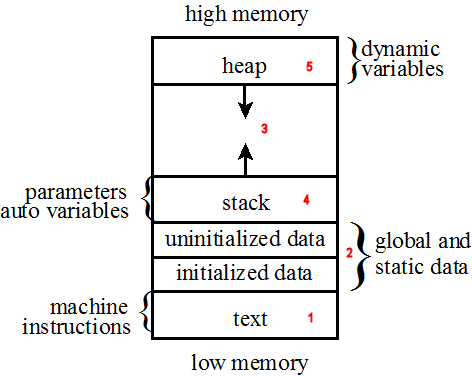
\includegraphics[width=0.5\textwidth]{images/memory_layout.png}
\caption{memory-layout}
\label{memory-layout}
\end{figure}

\subsection{const}
\subsection{stack and heap}
\subsection{Free Store}
\subsection{Global/Static}

\section{class}
\begin{lstlisting}
class derived_class : final base_class {
 public:
  derived_class() = default;
  derived_class & operator =( const derived_class & ) = delete;
  
  virtual void methods() final;	 //
};
\end{lstlisting}

\subsection{default}
类中的default关键字表示应该默认使用default部分定义的函数方法。当在class中定义某个方法为default属性时,编译器会自动为该方法创建一个对应的函数体实例化,不需要手动的来实现对应的函数内容,这在部分构造函数定义中十分有用,比如需要定义一套拷贝构造和赋值构造函数,一般的拷贝构造时比较麻烦的需要处理类里所有的成员变量等,但是使用default的话就可以让编译器默认来实现。
\begin{lstlisting}
class A {
 public:
  A(const A& rhs) = default;  // copy construct
  bool operator ==( const & A ) = default;
  bool operator !=( const & A ) = default;
  
 private:
  int data_;
};

// default same as:
A(const A& rhs) : data_(rhs.data_) {}

A aa;
auto a = aa;  // copy construct and initialize class a
\end{lstlisting}
拷贝构造是使用其他对象的值来初始化当前对象。注意是初始化类的时候对应等号左边的类是在拷贝构造的时候完成初始化的。赋值构造则是直接用一个新的对象来替换当前对象,赋值构造在调用的时候等号前后两个类都已经初始化完了,赋值构造完成赋值替换。
\begin{lstlisting}
class A {
 public:
  A& operator=(const A& rhs) = default;  // assignment construct

 private:
  int data_;
};
	
// default same as:
A& operator=(const A& rhs) {data_ = rhs.data_; return *this;}
	
A aa, a;  // a and aa already initialized.
a = aa;  // assignment construct
\end{lstlisting}

\subsection{delete}
类中使用delete修饰表示禁用对应的方法,编译器也不会自动实现对应的方法。使用delete的好处是在编译期就可以对代码进行规范性检查,如果有其他地方调用了delete的方法则会在编译器出错而不是到运行时出错。delete常用的是禁用拷贝构造:
\begin{lstlisting}
struct type {
 type & operator =( const type & ) = delete;
 type( const type & ) = delete;
};
\end{lstlisting}

使用delete完成模板的特化:
\begin{lstlisting}
// Delete primary class template, allow specializations
template<typename>
struct s = delete;
template<>
struct s<int> {
};

// Delete class specialization
template<typename>
struct t {
};

template<>
struct t<int> = delete;
\end{lstlisting}

使用delete来修饰析构函数,这种情况其实有点怪,因为一单析构函数被delete关键字修饰则对应的类不能够被析构掉。修饰析构函数一般是为了防止类中有申请的自由存储的内存等没有被释放的情况。比如:
\begin{lstlisting}
struct data {
  //...
};
	
struct data_protected {
 ~data_protected() = delete;
 data d;
};
struct data_factory {		
  ~data_factory() {
  for (data* d : data_container) {
	// this is safe, because no one can call 'delete' on d
	delete d;
	}
  }
		
  data_protected* createData() {
	data* d = new data();
	data_container.push_back(d);
	return (data_protected*)d;
  }

  std::vector<data*> data_container;
};
\end{lstlisting}

这里对结构体data\_protected,里面的data属性由于是new出来的,我们希望在特定的情况外部控制其释放。这样的话就最好禁用data\_protedted的析构函数使其一致存成,否则可能无法访问到对应的data成员。所以一般如果希望外部用户来控制对象的生命周期的话可以用delete。但是坏处是对应的类会一直存在。

\subsection{final}
\subsection{explicit}

\subsection{virtual}
\subsection{虚函数表}
\subsection{虚析构函数}
虚析构函数是为了解决基类的指针指向派生类对象,并用基类的指针删除派生类对象。如果基类析构函数不是virtual的,则无法通过基类指针删除派生类对象。
\begin{lstlisting}
class Base {
	public:
	Base() { std::cout << "construct base class.\n"; };
	virtual ~Base() { std::cout << "destroy base class\n"; }
};
class Derived : public Base {
	public:
	Derived() { std::cout << "construct derived class.\n"; }
	~Derived() { std::cout << "destroy derived class\n"; }
};

int main() {
	Base* method = new Derived();
	delete method;
	return 0;
}
// output:
// construct base class.
// construct derived class.
// destroy derived class
// destroy base class

// if Base destroy is not virtual, output is:
// construct base class.
// construct derived class.
// destroy base class
\end{lstlisting}
可以看出构造是先构造基类在构造派生类,析构是先析构派生类在析构基类。但是如果将基类析构函数设置为不是虚函数, 则派生类析构函数不会被调用,即派生类不会进行析构,从而导致内存泄露等问题。


\section{模板}
template代码的位置不能在.cpp/.cc之中,Templated code implementation should never be in a .cpp file: your compiler has to see them at the same time as it sees the code that calls them.一般都是放在.h文件中. 如果希望放在.cpp文件中要对class进行 explicit instantiation,对类模板A在.cpp最后加上:template class A;来实现显示生成object. 不能在class中特化模板;模板的定义一般是放在.h中,但是对该模板的特化定义要放在.cpp函数中.否则会有重定义的问题。模板只是代码的简化和宏展开一个效果,编译器会对每个类型都增加一个实现。不要在template中对某个特殊类型进行不同逻辑的处理,如果需要这样请特化。

\subsection{可选模板参数}
分析:
\begin{lstlisting}
template <typename T>
struct FUN {
	typedef int Type;
	...
}

template <typename T, typename = typename FUN<T>::Type>
void fun();
\end{lstlisting}
模板fun有两个模板参数一个是T另一个是typename = typename FUN$<$T$>::$Type,根据typename的Dependent names含义可以将fun简化为:
\begin{lstlisting}
template <typename T, typename = int>
void fun();
\end{lstlisting}
这里typename = 表示declaring template type parameters, 即需要定义一个模板变量。类模板定义的时候是可以指定一个默认值的。同时由于函数声明的时候函数名字可以省略,所以模板的第二个参数即定义了一个参数名字省略的int类型值。可以等价于:
\begin{lstlisting}
template <typename T, typename Type = int>
void fun();
	
template <typename T, int>
void fun();
\end{lstlisting}
这里用Type表示省略的名字,实际上相当于实现了一个偏特化的类,第二个模板参数是int。

\subsection{可变参数模板}
\subsection{Traits}

%% section for 
\section{多线程并发}

%% section for std
\section{std}
\subsection{std::vector}
\begin{lstlisting}
std::vector<int> nums1{};
std::vector<int> nums2{0, 1, 2, 3};
std::vector<int> nums3{0, 1, 2, 3, 4, 5};

size_t nums1_size = sizeof(nums1);   // 24
size_t nums2_size = sizeof(nums2);   // 24
size_t nums3_size = sizeof(nums3);   // 24
\end{lstlisting}
这里对std::vector求sizeof大小都是24个字节,这个大小不是vector存储的内容的大小,二是vector这个结构体存储的大小,24字节分别存储了三个指针: begin of vector, end if vector and end of reserved memory for vector。在64位系统上用8字节大小存储指针,比如:
\begin{lstlisting}
sizeof(int*) == sizeof(float*) == 8;
\end{lstlisting}
所以vector大小就是3*8=24字节。std::vector多了一个指向预分配内存的指针,如下:
\begin{lstlisting}
std::vector<int> nums;
nums.reserve(10);
nums[0] = 0;
std::cout << nums.size() << " " << nums.capacity() << "\n";   // 0, 10
nums.emplace_back(1);
std::cout << nums.size() << " " << nums.capacity() << "\n";   // 1, 10
nums.reserve(20);
std::cout << nums.size() << " " << nums.capacity() << "\n";   // 1, 20

int* data = nums.data();  // vector to data pointer
\end{lstlisting}
reserve会预分配给vector一个内存空间,会影响vector的capacity(最大可容纳元素的个数),但是不会影响size, 只有push\_back, emplace\_back会影响size大小。所以除了存储首地址和尾地址之外还需要一个指向其最大capacity处的地址指针。比如上面的nums,vector.begin()指向下标为0的元素,vector.end()是vector.begin() + vector.size(),指向末尾元素+1的位置,这里就是指向下标为1的元素(只有一个元素)。而剩下nums其实还有19个存放元素的内存大小。所以如果没有使用reserve预先分配内存,则vector每次push\_back元素的时候都会改变vector的申请内存的大小,会重复的释放和重新申请内存导致效率降低。如果reserve了一个size,但是实际使用的时候push的个数大于预先分配的尺寸,则vector会重新分配一个2倍reserve大小的内存大小。
\begin{lstlisting}
std::vector<int> nums;
nums.reserve(10);
nums.emplace_back(1);
std::cout << nums.size() << " " << nums.capacity() << "\n";   // 1, 10
for (int i = 0; i < 15; ++i) {
  nums.emplace_back(i);
}
std::cout << nums.size() << " " << nums.capacity() << "\n";   // 16, 20
\end{lstlisting}
如上,vector的capacity在push个数大于10个之后capacity的值从10变成了20。

\subsection{std::forward and std::move}
\textbf{std::forward}\newline
当输入是一个lvalue时, 匹配到如下模板。remove\_reference\_t会删除所有的reference,则输入相当于是\_Ty\&\ \_Arg。然后经过Reference collapsing(引用折叠)\_Ty\&\&\ \&\_Arg之后返回还是一个lvalue形式。
\begin{lstlisting}
template<class _Ty>
_NODISCARD constexpr _Ty&& forward(remove_reference_t<_Ty>& _Arg) noexcept
{	// forward an lvalue as either an lvalue or an rvalue
	return (static_cast<_Ty&&>(_Arg));
}
\end{lstlisting}
Reference collapsing规则是偶数引用可删除:\newline
\begin{itemize}
\item[$\bullet$] T\&\&\ \&\& → T\&\&
\item[$\bullet$] T\&\ \&\& → T\&
\item[$\bullet$] T\&\ \& → T\&
\item[$\bullet$] T\&\&\ \& → T\&
\end{itemize}
当输入是一个右值时,
\begin{lstlisting}
template<class _Ty>
_NODISCARD constexpr _Ty&& forward(remove_reference_t<_Ty>&& _Arg) noexcept
{	// forward an rvalue as an rvalue
	static_assert(!is_lvalue_reference_v<_Ty>, "bad forward call");
	return (static_cast<_Ty&&>(_Arg));
}
\end{lstlisting}

\subsection{std::enable\_if}
\subsection{std::find\_if}
\subsection{std::map和std::unordered\_map}
std::unordered\_map无序数组主要是通过hashmap来实现的,通过数组和链表hashmap定义可表示为:
\begin{lstlisting}
template <typename _Key, typename _Value>
struct HashNode {
	_Key key_;
	_Value value_;
	HashNode* next_;
};

template <typename _Key, typename _Value, class HashFun, class EqualFun>
struct HashMap {
 private:
  HashNode<_K, _Value>** hash_table;
  unsigned int size_;   // total hash map(hash_table) size
};
\end{lstlisting}
HashMap模板函数包括: \_Key一般是一个hashcode用来表示唯一的id信息,也可以是整数,string等。\_Value则表示需要存储的数据结构。hashmap的数据都存储在一个hash\_table中,hash\_table可以看出一个array或者vector。具有一定的大小(size\_),每个元素存储了一个链表的首节点地址指针。则对于任意一个map中的元素则可以通过整数索引来获取。那么如何获取这个整数索引呢?这就需要输入一个HashFun将\_Key转换成一个整数id,比如用下面函数:
\begin{lstlisting}
static int indexFor(int key, int max_size) {  
  return key & (max_size - 1);
}
\end{lstlisting}
这里如果key是一个int值,max\_size表示hash\_table的长度size\_,则通过求余数将一个很大的整形数或者hash值转换成到0到size\_之间的一个整数id。然后用id来从hash\_table中索引具体的节点HashNode。HashNode主要包含三个成员变量,key是hashcode值,表示当前node节点的唯一id值。value表示存储的整数数据结构体,next指针指向下一个HashNode节点。如果hash值映射的id都是唯一的,那么hash\_table的value就是每一个node节点的地址指针。但是这里就会出现可能会出现多个不同的hash值映射成了一个索引id(hash冲突),因为没有办法将size\_设置的很大来容纳所有的hash值,所以如果对于同一个id, 通过next指针指向下一个HashNode的形式多个node之间形成一个单链表,这些node的共同特点是其在hash\_table中的整数id都是同一个值,然后在基于链表逐个node去比较node中的key\_值和hashcode是否一样,一样则说明查找到了对应的数值,如果找不到说明是一个新的值,则基于输入的key和value新建一个node并插入到链表头中(因为hashtable中存储的是表头的地址指针)。HashMap通过数组和单链表的形式,获取到id之后只要最多遍历一遍链表就可以查找到对应的value,如果没有hash冲突,算法复杂度则为O(1),如果有则算法复杂度O(n)。另外当元素过少可以用单链表形式表示,但是元素过多的话则需要用红黑树来表示存储形式。

\subsection{std::queue and std::stack}
queue(队列)原则是元素先进先出,stack(栈)元素是后进先出。queue.pop()移除的是第一个进queue的元素,stack.pop()移除的是最后一个进stack的元素。
\begin{lstlisting}
std::queue<int> queue;
queue.push(0);
queue.push(1);
int first = queue.front();  // 0
queue.pop();  // remove first element

std::stack<int> stack;
stack.push(0);
stack.push(1);
int top = stack.top();   // 1
stack.pop();  // remove the top element
\end{lstlisting}

\subsection{std::sort}
std::sort可实现迭代排序功能,默认升序排序,也可以传入lambda函数来指定排序规则。sort会直接改变输入的迭代器里的值。当传入一个lambda排序函数时,lambda的两个输入表示比较迭代项的值,比如begin()指向的值。lambda必须返回一个bool值表示比较条件,如下a[1] < b[1]表示按照vector第2个元素升序排序,如果a的第二个值小a排在前面。
\begin{lstlisting}
#include <algorithm>  // std::sort

std::vector<int> vec1{2, 1, 3};
std::vector<std::vector<int>> vec2{{2, 1}, {1, 3}, {3, 0}};
std::sort(vec1.begin(), vec1.end());   // vec1: {1, 2, 3}
std::sort(vec2.begin(), vec2.end());   // vec2: {{1, 3}, {2, 1}, {3, 0}}, sort for first element
std::sort(vec2.begin(), vec2.end(), [&](std::vector<int>& a, std::vector<int>& b) { return a[1] < b[1]; });  // {{3, 0}, {2, 1}, {1, 3}}
\end{lstlisting}

%% section for cmake
\section{cmake}
\subsection{cmake demo}
\section{gcc}
\section{设计模式}

%%%%%%%%%%%%%%%%%%%%%%%%%%%%%%%%%%%%%%%%%%%%%%%%%%%%%%%%%%%%%%%%%%%%%%%%%%%%%%%%%%%%%%%%%%%%%%%%%%%%%%%%%
\newpage

\fancyhead{}
\fancyhead[CO,CE]{CUDA}

%\setcounter{chapter}{0}
\chapter{第八章\ CUDA}
\section{基础概念}
\subsection{Hello Add}
cuda编程的思想是并行多线程同时在cuda核上运行,一个cuda的加法demo如下:
\begin{lstlisting}
// cuda_add.cu
#include <cuda_runtime.h>

__global__ void cuda_add(float* A, float* B, float* C)
{
  int block_idx = blockIdx.x;
  int thread_idx = threadIdx.x;
  int blockdim = blockDim.x;
  int idx = block_idx * blockdim + thread_idx;
  C[idx] = A[idx] + B[idx];
}

int main()
{
  #define BLOCK_SIZE 64
  
  int N = 1000;
  size_t nBytes = N * sizeof(float);

  float *h_A, *h_B, *h_C;
  h_A = (float*)malloc(nBytes);
  h_B = (float*)malloc(nBytes);
  h_C = (float*)malloc(nBytes);
  // ...
  
  float *d_A, *d_B, *d_C;
  cudaMalloc((float**)&d_A, nBytes);
  cudaMalloc((float**)&d_B, nBytes);
  cudaMalloc((float**)&d_C, nBytes);
  
  cudaMemcpy(d_A, h_A, nBytes, cudaMemcpyHostToDevice);
  cudaMemcpy(d_B, h_B, nBytes, cudaMemcpyHostToDevice);
  
  cudaSetDevice(0);
  dim3 dimBlock(BLOCK_SIZE);
  dim3 dimGrid((N + BLOCK_SIZE - 1)/ BLOCK_SIZE);
  cuda_add<<<dimGrid, dimBlock>>>(d_A, d_B, d_C);
  cudaDeviceSynchronize();  // wait gpu compute end
  cudaMemcpy(h_C, d_C, nBytes, cudaMemcpyDeviceToHost);

  free(h_A);
  free(h_B);
  free(h_C);

  cudaFree(d_A);
  cudaFree(d_B);
  cudaFree(d_C);
}
// compiler:
// nvcc cuda_add.cu -o cuda_add
\end{lstlisting}
一个cuda核用\_\_global\_\_关键字来定义,cuda\_add执行通过$<<<...>>>$操作符来定义,dimGrid和dimBlock定义了具体的线程数配置。一组的线程组成了cuda block, cuda block组成了cuda grid。一个二位cuda grid可视化:
\begin{figure}[H]
	\centering
	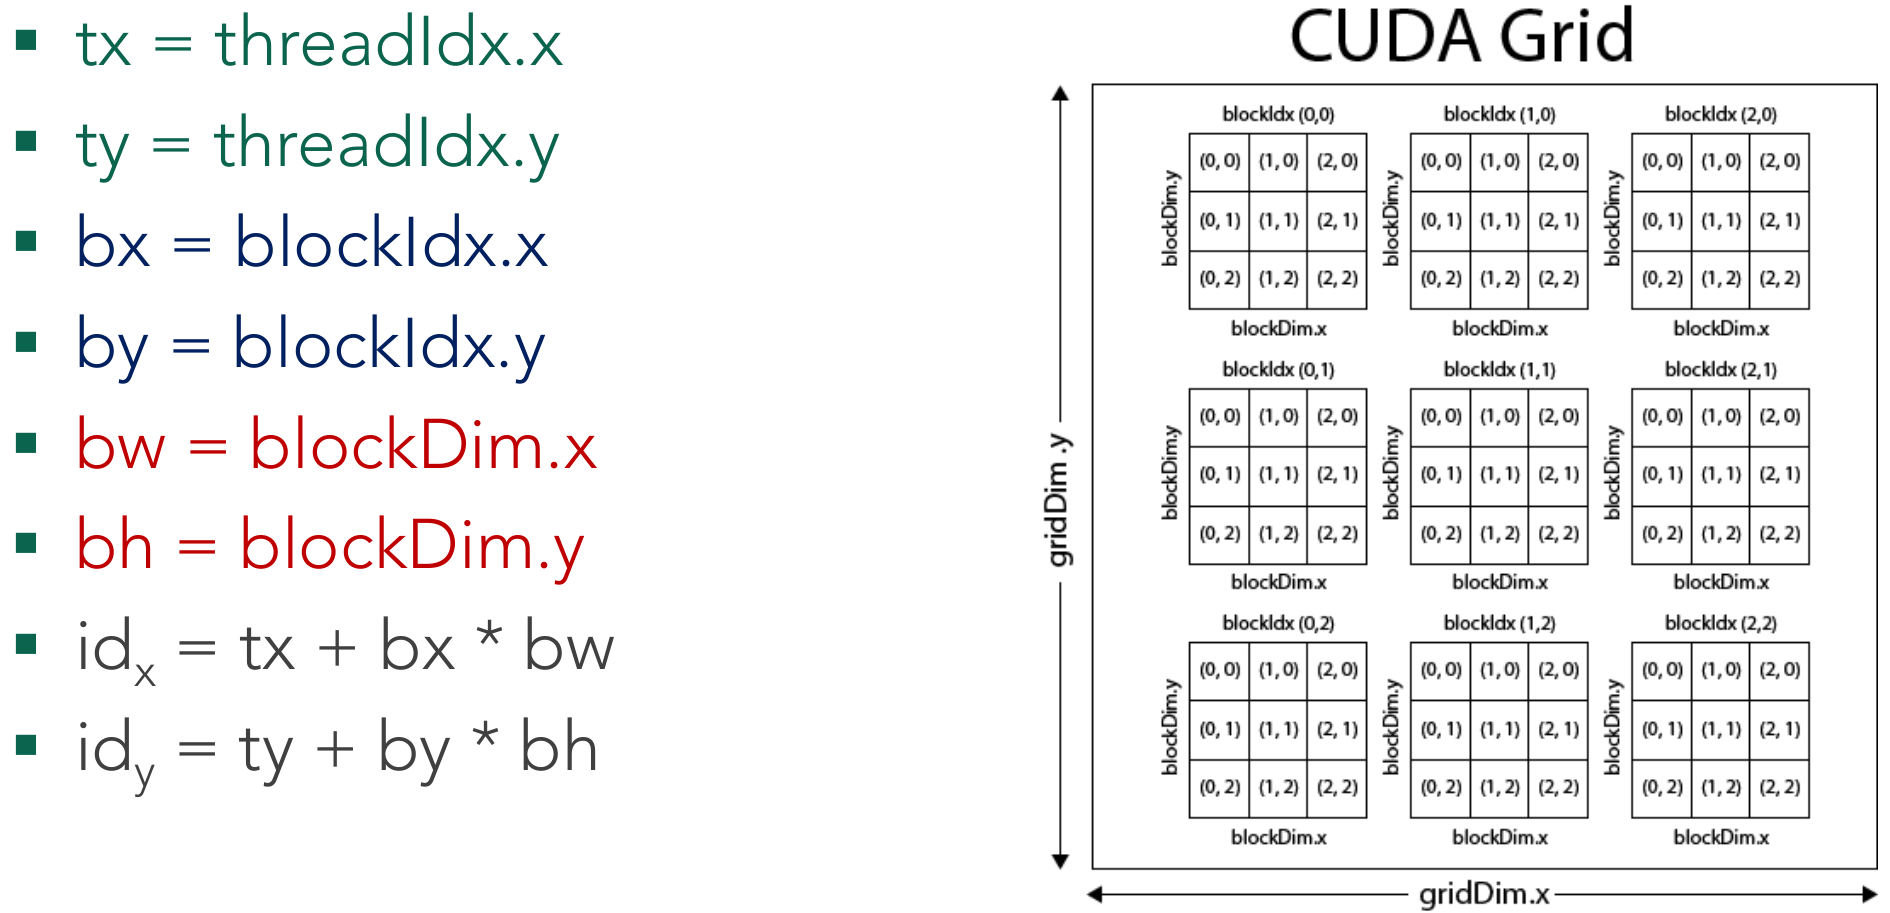
\includegraphics[width=0.9\textwidth]{images/cuda_grid_block.png}
	\caption{cuda-grid}
	\label{cuda-grid}
\end{figure}
如cuda\_add中定义BLOCK\_SIZE表示一个cuda block的大小是多少。在定义dimGrid和dimBlock的时候其实都是dim3是3个维度的,即dimx, dimy, dimz。当不指定其他两个维度,大小默认是1。所以$ dimBlock(BLOCK\_SIZE);$相当于$dimBlock(BLOCK\_SIZE, 1, 1);$,即blockDim.x = BLOCK\_SIZE, blockDim.y == blockDim.z == 1。同理dimGrid为:
\begin{equation}\label{compute-dim-grid}
dimGrid = (N + BLOCK_SIZE - 1) / BLOCK_SIZE;
\end{equation}
这种就发可以保证dimGrid * dimBlock可以将所有的输入数据N都包含在内,比如N是1000, dimBlock是64,则dimGrid是16。这里只考虑x一个维度,即使用16个cuda block(gridDim.x = 16), 每个cuda block的大小是64(blockDim.x = 64)。所以一共有1024个线程在同时计算,每个线程的索引可以通过:
\begin{equation}\label{compute-cuda-thread-idx}
int\ idx = blockIdx.x * blockDim.x + threadIdx.x;
\end{equation}
其中blockIdx.x,blockDim.x,threadIdx.x都是cuda函数内置的一些变量,表示当前线程核函数的信息: blockIdx.x表示当前线程属于哪一个block,范围在0到gridDim.x-1之间。blockDim.x:一个常数通过表示x维度一个block包含了多少个线程。threadIdx.x: 当前block内这个cuda kernel的线程索引是多少,范围属于0到blockDim.x-1。然后这里每个线程进行两个数的相加操作。那么cuda kernel和设备对应关系是什么呢?如下图对于GPU设备是由很多个Multithreaded Streaming Multiprocessors (SMs)组成的,图中一个绿色格表示一个core core,多个cuda core组成了一个SM。这里一个SM包含32个cuda core,一个GPU设备含有8个SMs。
\begin{figure}[H]
	\centering
	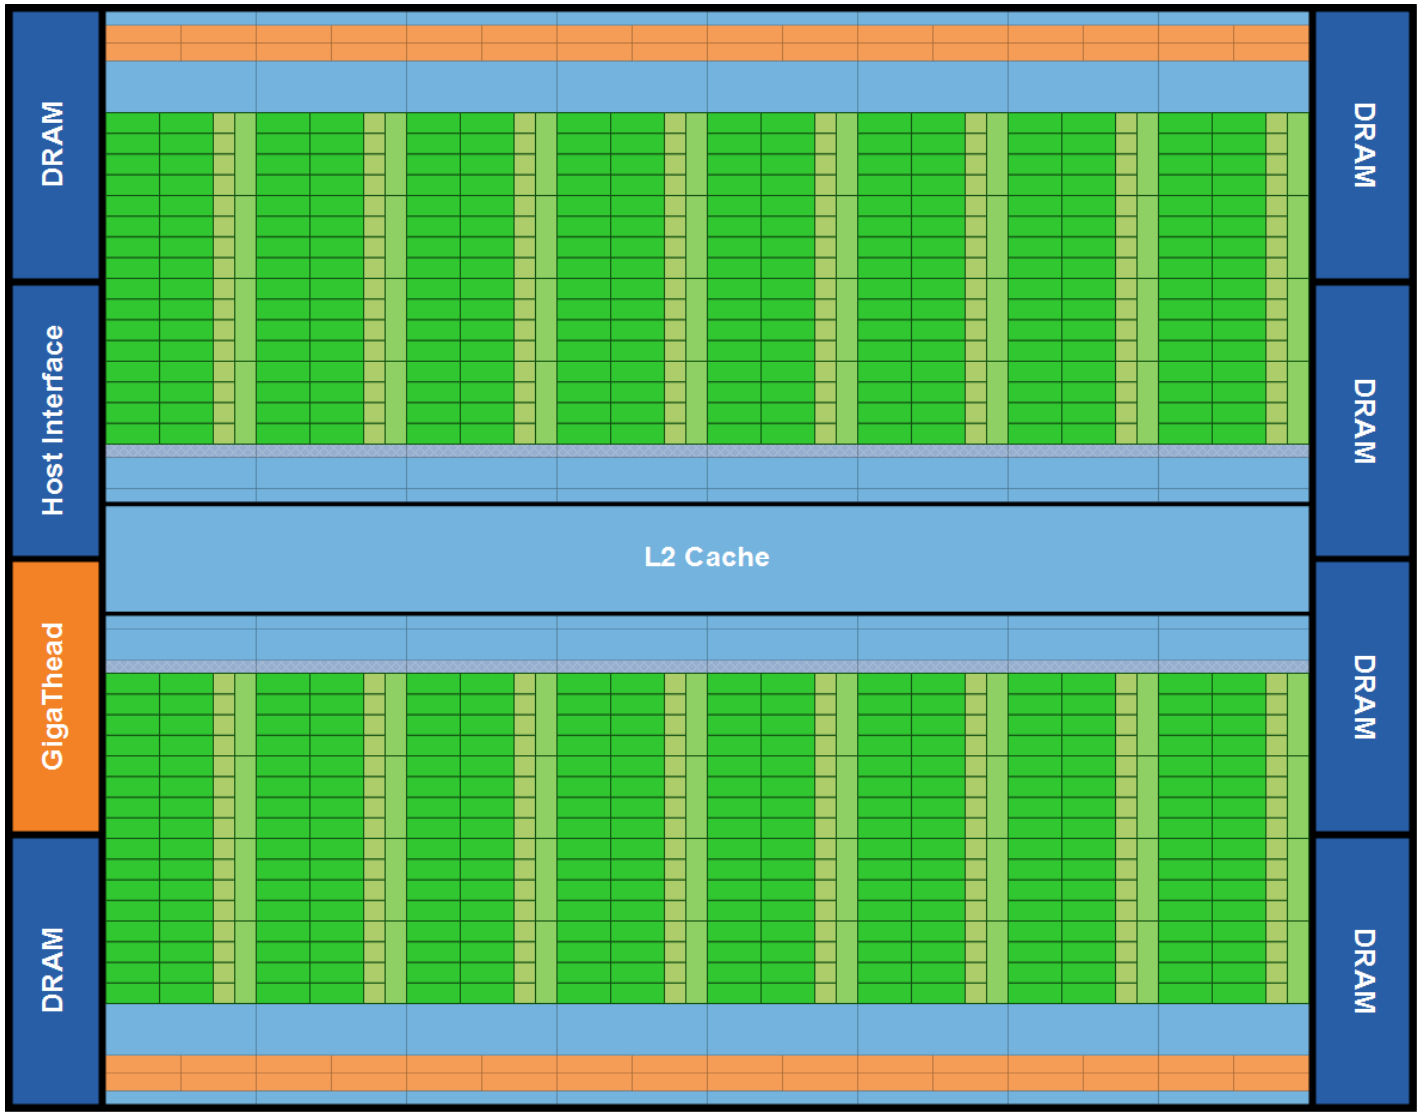
\includegraphics[width=0.9\textwidth]{images/GPU-Architecture.png}
	\caption{GPU-Architecture}
	\label{GPU-Architecture}
\end{figure}
一个SM的结构如下,cuda core (也称为Stream Processors (SP))最基本的计算单元,一个core core具有浮点计算单元和整形计算单元。当一个cuda kernel被执行时,会根据线程数目将cuda grid分配到不同的SM上去执行,但是对于一个cuda block来说只能在一个SM上执行。一个SM的CUDA core会分成几个warp(线程束),即CUDA core在SM中分组,一个warp中的线程必然在同一个block中,由于warp的大小一般为32,所以block所含的thread的大小一般要设置为32的倍数。一个cuda core可以运行16个线程,两个cuda core就可以组成一个线程束。
\begin{figure}[H]
	\centering
	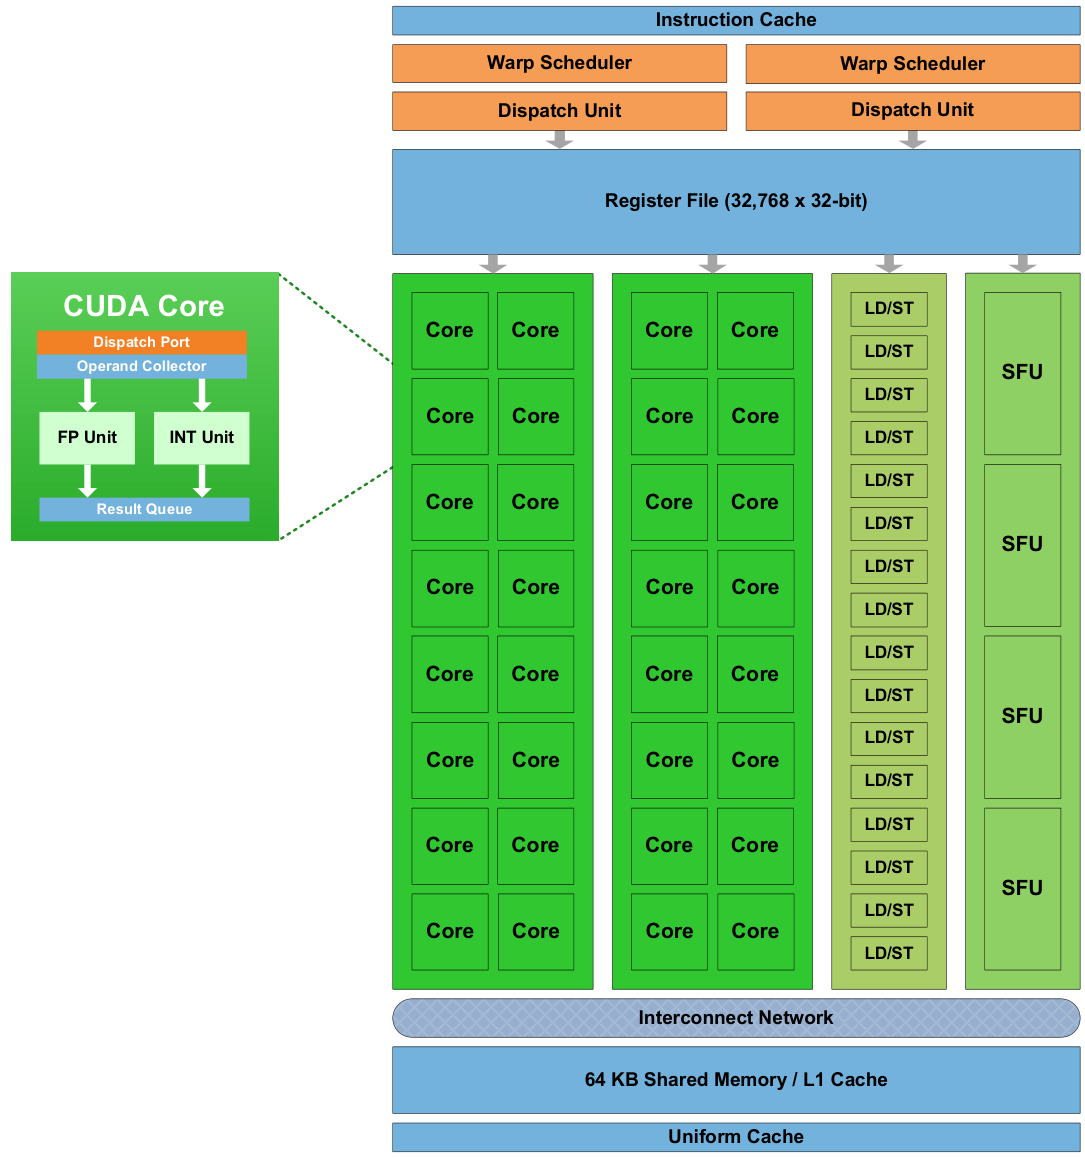
\includegraphics[width=0.9\textwidth]{images/cuda-one-sm.png}
	\caption{SM}
	\label{SM}
\end{figure}

\section{keyword}
\subsection{\_\_syncthreads}
\_\_syncthreads()用于线程间通信,保证block内所有线程都运行到调用\_\_syncthreads()的地方,然后在继续往下执行。
%%%%%%%%%%%%%%%%%%%%%%%%%%%%%%%%%%%%%%%%%%%%%%%%%%%%%%%%%%%%%%%%%%%%%%%%%%%%%%%%%%%%%%%%%%%%%%%%%%%%%%%%%
%%  参考文献  %%
\newpage
 
\fancyhead{}
\fancyhead[CO,CE]{参考文献}
 
\bibliographystyle{plain}
 
\chapter{参考文献}
\bibliography{reference.bib}

 
\end{document}